\documentclass[9pt,twocolumn,twoside]{styles/osajnl}
\usepackage{fancyvrb}
\journal{i524} 

\title{An Overview of OpenNebula Project and its Applications}

%\author[1,2,3]{John Smith}
%\author[2]{Alice Smith}
%\author[1]{Bruce Wayne}
\author[1]{Veera Marni}

\affil[1]{School of Informatics and Computing, Bloomington, IN 47408, U.S.A.}
%\affil[2]{School of Science, University of Technology, 2000 J St. NW, Washington DC, 20036}
%\affil[3]{School of Optics, University of Technology, 2000 J St. NW, Washington DC, 20036}

\affil[*]{Corresponding authors: vmarni@umail.iu.edu}

%\dates{project-000, \today}
\dates{\today}

\ociscodes{opennebula, open cloud, cloud computing}

% replace this with your url in github/gitlab
\doi{\url{https://github.com/narayana1043/sp17-i524/blob/master/paper1/S17-IR-2017/report.pdf}}


\begin{abstract}
This paper provides insight into how OpenNebula can provide the right 
cloud for unique needs of each organization. Down the line some real 
world applications are also discussed where OpenNebula has been 
successfully deployed.\newline
\end{abstract}

\setboolean{displaycopyright}{true}

\begin{document}

\maketitle

\section{Introduction} 

{OpenNebula}\cite{www-wiki-opennebula}is a open cloud platform 
using which each organization setup the right cloud for its 
organizational needs. This quite natural like it happened with the 
databases and web-servers. {As one cloud could not solve all the 
needs of various work environments OpenNebula helps in setting up and 
deploying cloud platform based on needs}\cite{www-about-opennebula}. 
It is a simple feature rich and flexible solution for the management 
of virtualized data centers.

It's interoperability makes cloud progress in developments of new 
methodologies to take advantage of the IT assets in turn saving 
investments and completely avoiding lock-in costs for the project. 
It's platform manages a data center's virtual infrastructure to build 
private, public and hybrid implementations of infrastructure as a 
service. It is a trunkey enterprise-ready solution that includes all 
features need to provide private and public cloud services. It is a 
open cloud architecture which is simple, open, reliable and 
flexible. 

The paper is organized as follows. First OpenNebula's Architecture is 
discussed followed by Integration, API's and Language Binding. It is 
then followed by OpenNebula ecosystem and licensing. Finally, use 
cases are discussed with respect to its intended users which followed 
by key features and educational resources. It is then concluded by 
high lighting the major drawbacks that need attention in moving 
forward.


\section{Architecture of OpenNebula}

OpenNebula is a cloud computing platform for managing heterogeneous 
distributed data center  infrastructures. The OpenNebula platform 
manages a data center's virtual infrastructure to build private, 
public and hybrid implementations of infrastructure as a service. It 
provides features at two main layers of Data Center Virtualization 
and Cloud Infrastructure.

\begin{figure}[htbp]
	\centering
	\fbox{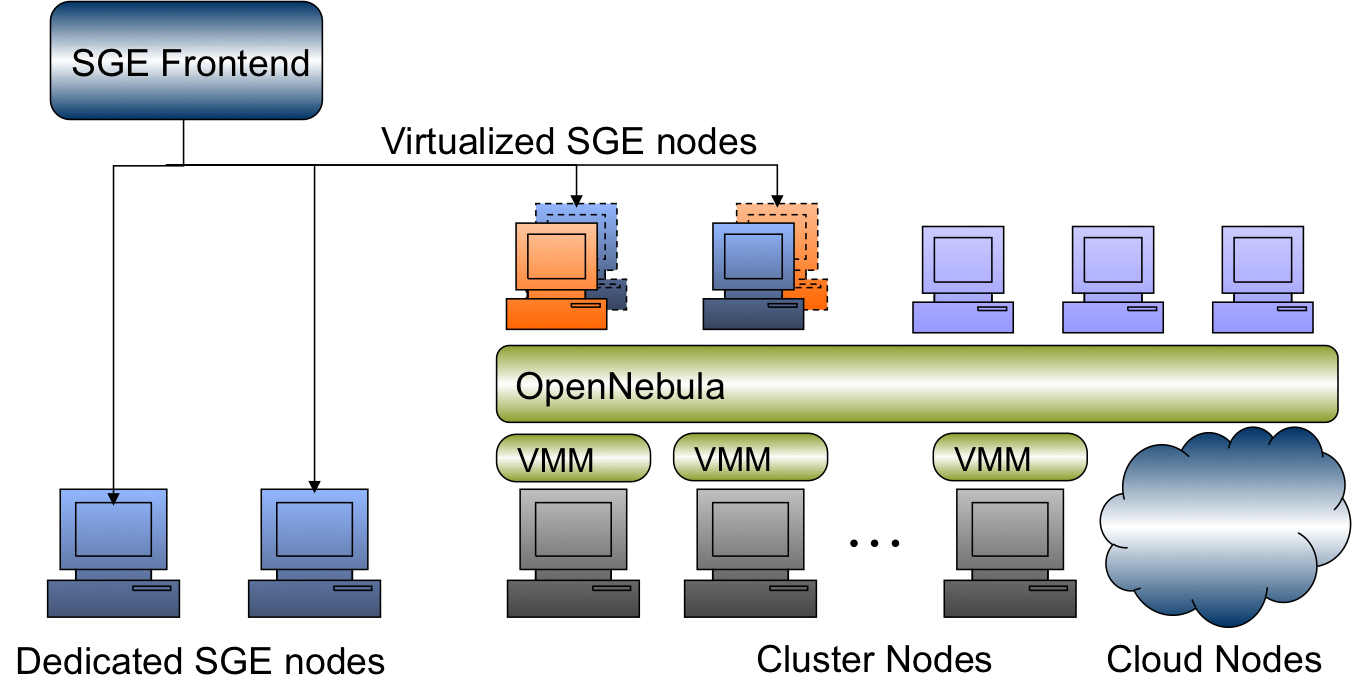
\includegraphics[width=\linewidth]{images/functionality.png}}
	\caption{The OpenNebula Engine for Data Center Virtualization and 
		Cloud Solutions.}
	\label{fig:false-color}
\end{figure}

\subsection{Data Center Virtualization Management}

Many users use OpenNebula to manage {data center 
virtualization}\cite{www-dcv-opennebula}, 
consolidate servers, and integrate existing IT assets for computing, 
storage, and networking. In this deployment model, OpenNebula 
directly integrates with hyper-visors and has complete control over 
virtual and physical resources, providing advanced features foe 
capacity management, resource optimization, high availability and 
business continuity.

\subsection{Cloud Management}

OpenNebula also provides a multi-tenant, cloud-like provisioning 
layer on top of an existing infrastructure management solution (like 
VMware vCenter). It helps in provisioning, elasticity and 
multi-tenancy cloud features like virtual data centers provisioning, 
data center federation or hybrid cloud computing to connect in-house 
infrastructure is managed by already familiar tools for 
infrastructure management and operation. 

\section{Integration, API's and Language binding}

\subsection{System Interfaces}
OpenNebula has been designed to be easily adapted to any 
infrastructure and easily be extended with new components. The result 
is a modular system that can implement a variety of cloud 
architectures and can interface with multiple data center services. 
It interfaces can be classified into e categories

\begin{enumerate}
	\item end-user cloud interfaces
	\item system interfaces
\end{enumerate}

Cloud interfaces are primarily used to develop tools to the end-user, 
and they provide a high level abstraction of the functionality 
provided by the cloud. They are designed to manage virtual machines, 
networks and images through a simple and easy-to-use REST API. The 
clod interfaces hide most of the complexity of a cloud and specially 
suited for end-users. OpenNebula features a EC2 interface, 
implementing the functionality offered by the Amazon's EC2 API, 
mainly those related to virtual machine management. In this way, you 
can use any EC2 Query tools to access your OpenNebula Cloud.

{System interfaces}\cite{www-opennebula-systeminterfaces} expose the 
full functionality of OpenNebula and are 
mainly used to adapt and tune the behavior of OpenNebula to the 
target infrastructure. The XML-RPC interface is the primary interface 
for OpenNebula, exposing all the functionality to interface the 
OpenNebula daemon. The OpenNebula cloud API provides a simplified and 
convenient way to interface with the OpenNebula core XMLRPC API. 
OpenNebula also includes 2 language bindings for OCA: Ruby and JAVA. 
The OpenNebula OneFlow API is a RESTful service to create, control 
and monitor service to create, control and monitor services composed 
of interconnected VMs with deployment dependencies between them.

\subsection{Infrastructure Integration}

The interactions between OpenNebula and the {Cloud 
infrastructure}\cite{www-opennebula-infraintegration} are 
performed by specific drivers. Each one addresses a particular area:

\textbf{Storage} The OpenNebula core issue abstracts storage 
operations that are implemented by specific programs that can be 
replaced or modified to interface special storage back-ends and file 
systems.

\textbf{Virtualization} The interaction with the hypervisors are also 
implemented with custom programs to boot, stop or migrate a virtual 
machine. This allows you to specialize each VM operation so to 
perform custom operations.

\textbf{Monitoring} Monitoring information is also gathered by 
external probes. You can add additional probes to include custom 
monitoring metrics that can later be used to allocate virtual 
machines or for accounting purposes.

\textbf{Authorization} OpenNebula can be also configured to use an 
external program to authorize and authenticate user requests. In this 
way, you can implement any access policy to Cloud resources.

\textbf{Networking} The hypervisor is also prepared with the network 
configuration for each Virtual Machine.

\section{Ecosystem}

The {OpenNebula Ecosystem}\cite{www-opennebula-ecosystem} is formed 
by external tools and extensions 
that complement the functionality provided by the OpenNebula Cloud 
Management Platform. In addition, the ecosystems built around the 
cloud interfaces implemented by OpenNebula, Amazon AWS and OGC OCCI, 
can also be leveraged. 

\section{Use Cases of OpenNebula}

\subsection{For the Infrastructure Manager}

OpenNebula responds quickly to infrastructure needs for services with 
dynamic resizing of the physical infrastructure by adding new hosts 
and dynamic cluster partitioning to meet capacity requirement of 
services. It has centralized management of all the virtual and 
physical distributed infrastructure. It can improve the utilization 
of existing resources in the data center and infrastructure sharing 
between different departments managing their own production clusters, 
so removing application silos. It improves operational saving with 
server consolidation to a reduced number of physical systems, so 
reducing space, administration efforts, power and cooling 
requirements. It has also reduced infrastructure expenses with the 
combination of locate and remote cloud resources so eliminating the 
over purchase of systems to meet peak demands.

\subsection{For the Infrastructure user}

It is built for fast delivery and scalability of services to meet 
dynamic demands of service end-users. It supports heterogeneous 
execution environment with multiple, even conflicting, software 
requirements on the same shared infrastructure. It also provides full 
control of the life cycle of virtualized services management.

\subsection{For System Integrators}

It fits into any existing data center due to its open, flexible and 
extensible interfaces, architecture and components. It can build any 
type of cloud deployment. It is open sourced under Apache license and 
has seamless integration with any product and service in the 
virtualization/cloud ecosystem and management tool in the data 
center.

\section{Key Features and Components OpenNebula}

\subsection{Features}
There are several key {features of 
OpenNebula}\cite{www-features-opennebula} for the comprehensive 
management of virtualized data centers to enable private, public and 
hybrid clouds. Some of these key features are interfaces for cloud 
consumers, service management and catalog, interfaces for 
administrators and advanced users, appliance market place, 
chargeback, capacity and performance management, high availability 
and business continuity, virtual infrastructure management and 
orchestration, external cloud connector, platform independent, 
security, integration with third-party tools, fully open-sourced, 
automatic upgrade process, quality assurance and community support.

\subsection{Components}

OpenNebula has several {advanced components}\cite{www-components} 
that can be easily 
integrated and deployed. Some of the important components that are 
extensively used are listed below:

\begin{enumerate}
	
	\item Multi-VM Applications and Auto-scaling
	\item Host and VM Availability
	\item Data Center Federation
	\item Cloud Bursting
	\item Application Insight
	\item Public Cloud
	\item MarketPlace
	
\end{enumerate}

\section{Educational Material}

A great place to start is by reading the {OpenNebula 
documentation}\cite{www-opennebula-documentation}. 
{Future Systems has a tutorial on there 
webpage}\cite{www-opennebula-tutorial} to get started with 
OpenNebula. {Handbook of Research on High Performance and Cloud 
Computing in Scientific Research and Education}\cite{book-hpc} by 
Marijana Despotovic-Zrakic is great book to get started from the 
basics of cloud computing and understanding the working of OpenNebula.

\section{Conculsion}

OpenNebula is made impact in the way cloud services are offered 
before it was introduced by reducing costs of infrastructure, 
increasing the utilization of available resources, increase the 
computing power by integrating different machines and simplifying the 
development and deployment in industry. However, there are some 
disadvantages that needs attention. Some of them are Greater 
dependency on service providers, Risk of being locked into 
proprietary or vendor-recommended systems, Potential privacy and 
security risks of putting valuable data on someone else's system. 
Another important problem what happens if the supplier suddenly stops 
services. Even with this disadvantages the technology is still used 
greatly in various industries and many more are looking forward to 
move into cloud.

\bibliography{references}

\end{document}
